\documentclass[12pt]{article}

\usepackage{amsmath,amsfonts,amssymb}
\usepackage[utf8]{inputenc}
\usepackage{microtype}
\usepackage{copyrightbox}

\title{Mastering Chess and Shogi by Self-Play with a General Reinforcement
Learning Algorithm: Implementation Report}
\author{
    Aamr \textsc{El Kazdadi}\\
    Ahmed \textsc{El Alaoui Talibi}\\
    El Mahdi \textsc{Chayti}}
\date{}
\begin{document}
\maketitle

\section{Introduction}
AlphaZero is an algorithm designed to master the games of Go, chess and shogi,
by \textit{tabula rasa} reinforcement learning. This is accomplished by
using a neural network to estimate the best moves, and training the neural
network through repeated self play.

\pagebreak
\section{General idea of the approach}
\begin{figure}[h!]
    \centering
    \copyrightbox[r]
    {
        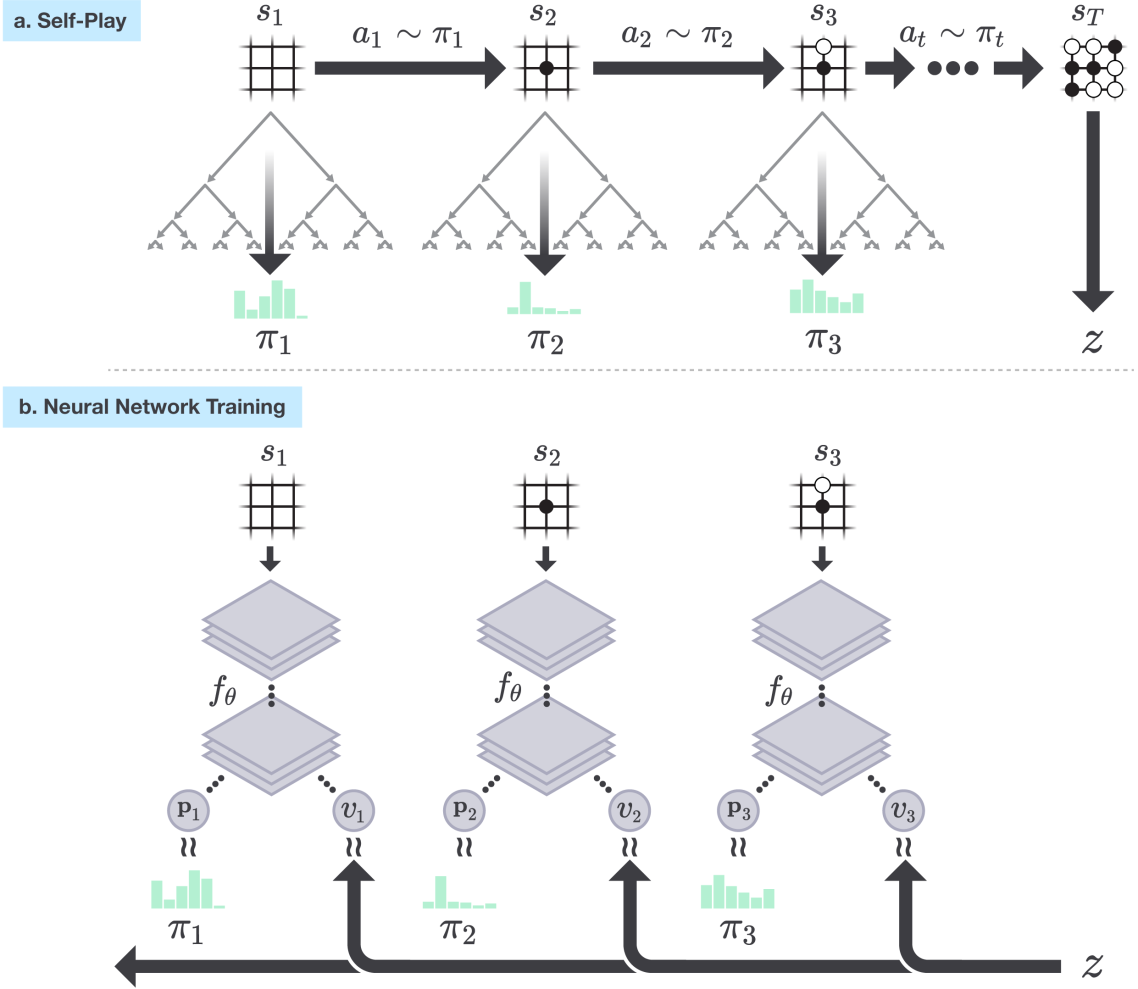
\includegraphics[width=.9\textwidth]{plots/method.png}
    }
    {\textcopyright Mastering the Game of Go without Human Knowledge - DeepMind}
    \caption{Self-play reinforcement learning in AlphaZero}
\end{figure}

The reason a deep learning approach is used for this task is because the state
space of the games is too large to enumerate. And so the value and policy
functions are estimated using a neural network, that takes as an input the
state of the game as a bit vector, and outputs $v(s)$, the estimated value of
the state and $f(s)$ a prior probability that roughly evaluates how strong the
neural network considers each legal move to be.

The program doesn't use these probabilities directly to choose its next move.
Instead, it executes a Monte Carlo Tree Search before taking action. And uses
the prior probabilities of the neural network to guide its move exploration,
as we will detail further down. The MCTS tends to output a much better policy
than the raw probabilities $f(s)$ of the neural network.

\section{Monte Carlo Tree Search}
\begin{figure}[h!]
    \centering
    \copyrightbox[r]
    {
        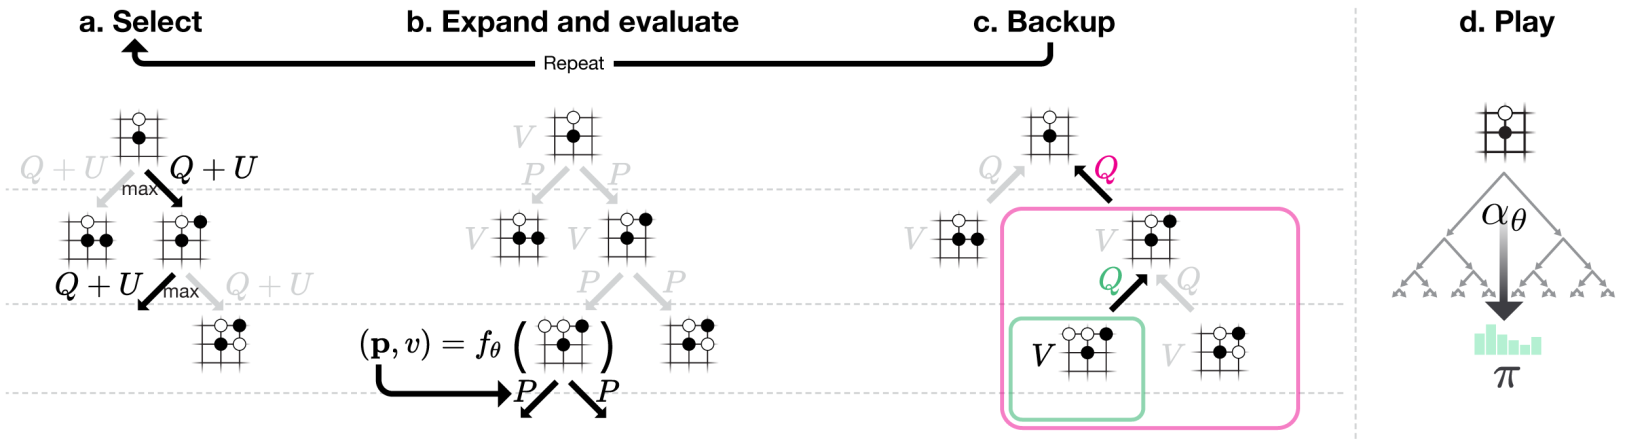
\includegraphics[width=.9\textwidth]{plots/mcts.png}
    }
    {\textcopyright Mastering the Game of Go without Human Knowledge - DeepMind}
    \caption{Monte Carlo Tree Search in AlphaZero}
\end{figure}

This search functions as a powerful \textit{policy improvement} operator, and
defines a stronger policy $\pi(s, a)$, proportional to the number of times
the action $a$ was used from state $s$ during the MCTS.

A MCTS is performed by building a tree, with the current state at the root.
We repeatedly navigate the tree, starting at the root, and choosing the actions
so as to maximize a quantity $Q(s,a) + U(s,a)$, where:
\begin{itemize}
    \item $Q(s,a)$ is the estimated value of a given action $a$ from the state
        $s$, given by the average of the values that were propagated up the
        tree.
    \item $U(s,a) = C_{\text{puct}} p_\theta(s,a)\frac{\sqrt{\sum_b
        N(s,b)}}{1+N(s,a)}$
    \item $N(s,a)$ is the number of times action $a$ was taken from state $s$
        so far.
    \item $C_{\text{puct}}$ controls the exploration rate.
    \item $p_\theta(s,a)$ is the neural network's policy. The raw probability
        of taking action $a$ from the state $s$.
\end{itemize}


Once a leaf node is reached, we check whether it's a terminal node (i.e., the
game is over) or not.
In which case, the value of the leaf node is set to $1$ if the current player
won, $-1$ if lost, and $0$ in the case of a draw.

If the state is not terminal, we typically simulate the rest of the game
and use the result to determine its value.

However, the AlphaZero algorithm uses a variant of the MCTS, where instead
of simulating the entire game, we estimate the value of the node's state
using the given neural network.
Its actions and the states they lead to are added to the tree as children of
the leaf, and the value of the leaf along with the prior probabilities
$p_\theta(s, \cdot)$ of the actions are estimated by the neural network.

In both cases, the value $v$ of the leaf node is then propagated along the path
that was taken from the root until it was reached. For each visited node $s$ on
the path from the root to the leaf, let $a$ be the action taken from $s$.
\\
We update the value $Q_{\text{new}}(s,a) = \frac{n}{n+1}Q(s,a) + \frac1{n+1}
\epsilon v$, and increment the number of visits $N(s,a)$ by 1.
\\
Here, $\epsilon$ is set to $1$ if the player taking action during the node $s$
is the same as the one in the leaf node, and $-1$ otherwise.

Once the root node is reached, we repeat the process of going down the tree
according to the actions maximizing $Q+U$ until a leaf is reached, then
updating the values.

After a certain number of iterations, we return the improved policy of the root
node's state, $p_\text{MCTS}(s, a)$, which is proportional to the number of times
action $a$ was taken during the MCTS procedure.

\section{Episode simulation}
Episodes are generated by pitting two player models against each other. We'll
refer to the model we wish to improve as the player, and the other one as the
opponent.

During each turn of the player, it generates an improved policy for the current
state using a MCTS. Then we transform the state and policy respectively into an
input and output adapted to the dimensions of the neural network, for training
purposes.

The neural network's output also contains the value of a given input
state. But that value is left blank until the game is over. It is then set
depending on the outcome of the game.

The action to be taken by the player is then chosen randomly according to the
probability distribution of the improved policy.

During the opponent's turn, the action is selected in a similar fashion, using
its own neural network in the MCTS procedure when needed, then choosing
randomly according to the improved policy.

\section{Model training}
We initialize a model with predefined or random weights to serve as the player,
and a second model to serve as the opponent, with a cloned architecture and
weights.

To improve the performance of our model its strategy. We generate a dataset
containing the inputs and outputs number of a number of episodes. We then
train the player's neural network according to the loss function:
\[
    L(\theta) = \sum_i (z_i - v_{\theta}(s_i))^2 - \pi_i(\cdot)^\top \log p_{\theta}(s_i, \cdot) + c \lVert \theta \rVert^2,
\]
where:
\begin{itemize}
    \item $v_\theta(s_i)$ is the value of state $s_i$ estimated by the neural
        network.
    \item $p_\theta(s_i, \cdot)$ is the policy vector of the actions of state
        $s_i$ estimated by the neural network.
    \item $z_i$ is the outcome of the game containing the state $s_i$.
    \item $\pi_i(\cdot)$ is the improved policy, found by the MCTS seach.
\end{itemize}

After the training is over, the process is repeated until the player achieves
a winrate higher than some threshold, typically chosen as $55\%$, after which
the model's weights are copied into the opponent's neural network, and the
process is repeated.

\section{Application}
We've implemented a general use algorithm that can play any game turn based
deterministic 2 player game, given the appropriate interface. And we provide
implementations for the games of tic-tac-toe, Connect Four and chess.

While the algorithm can reach superhuman performance in any game in theory,
given enough time, it requires an enormmous amount of computational power
for any non-trivial game.

As such, we limit ourselves to the game of tic-tac-toe, where we compare
the training procedure using different hyperparameters.

In the following figures, the blue, green and red areas represent the
percentage of wins, draws and losses respectively in the generated dataset.
The black curve plots the winrate in each one. And the shaded horizontal
line is the winrate threshold, which when surpassed, updates the weights
of the old model's neural network.

\begin{figure}[h!]
    \centering
    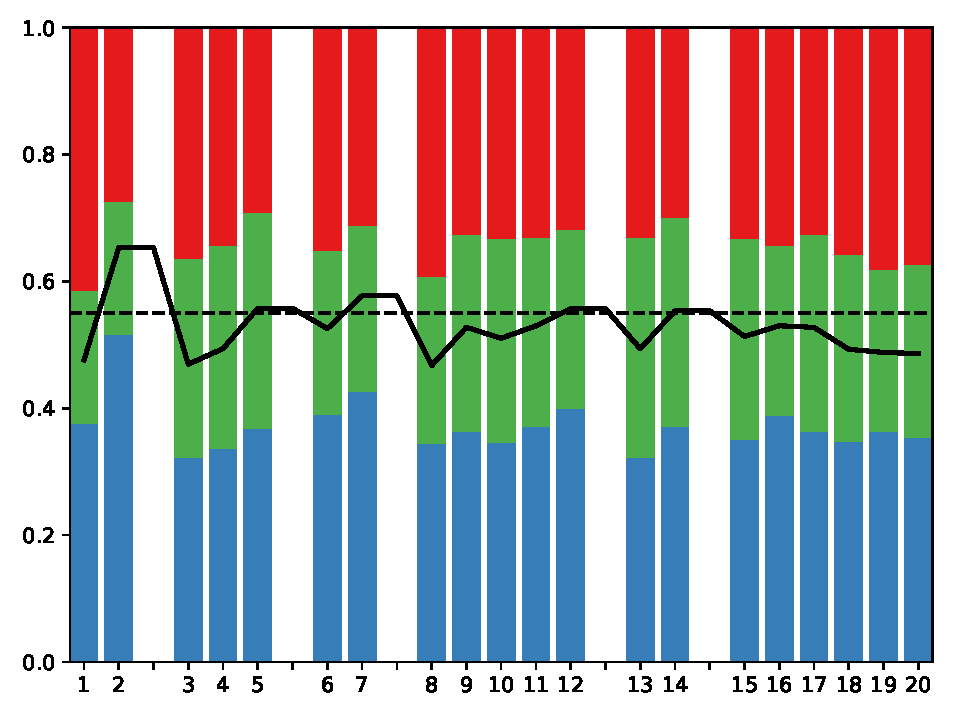
\includegraphics[width=.5\textwidth]{plots/0.pdf}
    \caption{500 episodes, 100 MCTS iterations}
\end{figure}

With a decently sized dataset and a large number of MCTS iterations, the model
improves progressively. Making small incremental improvements until it reaches
its optimal state.

\begin{figure}[h!]
    \centering
    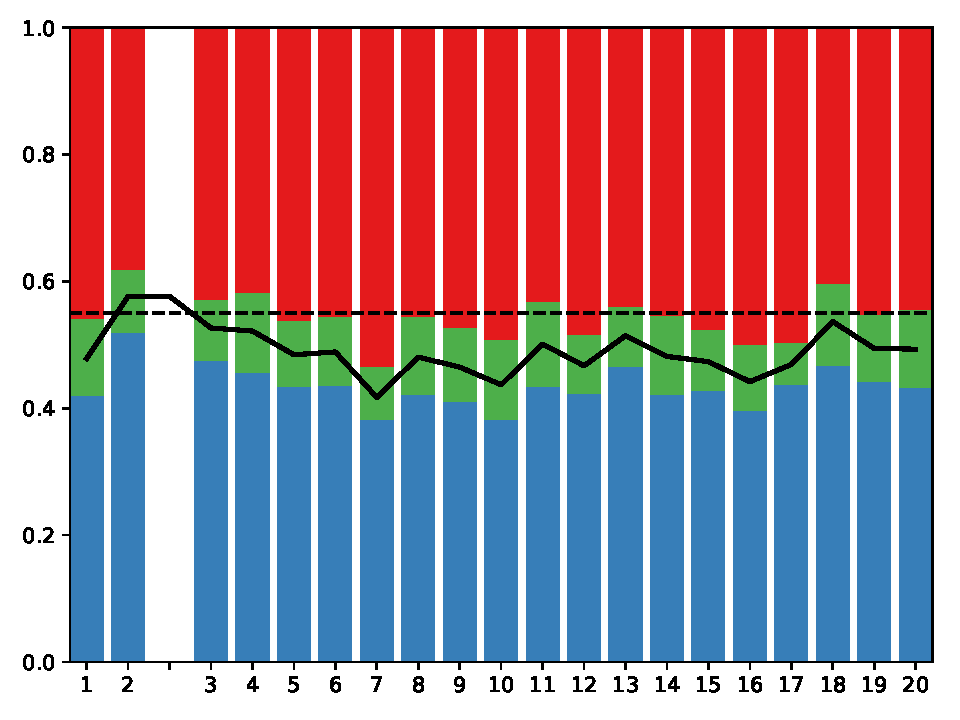
\includegraphics[width=.5\textwidth]{plots/2.pdf}
    \caption{500 episodes, 25 MCTS iterations}
\end{figure}

When the number of MCTS iterations is too low, the model tends to learn very
slowly, and is in fact not much stronger than it was, initially, and has
difficulty improving.

\begin{figure}[h!]
    \centering
    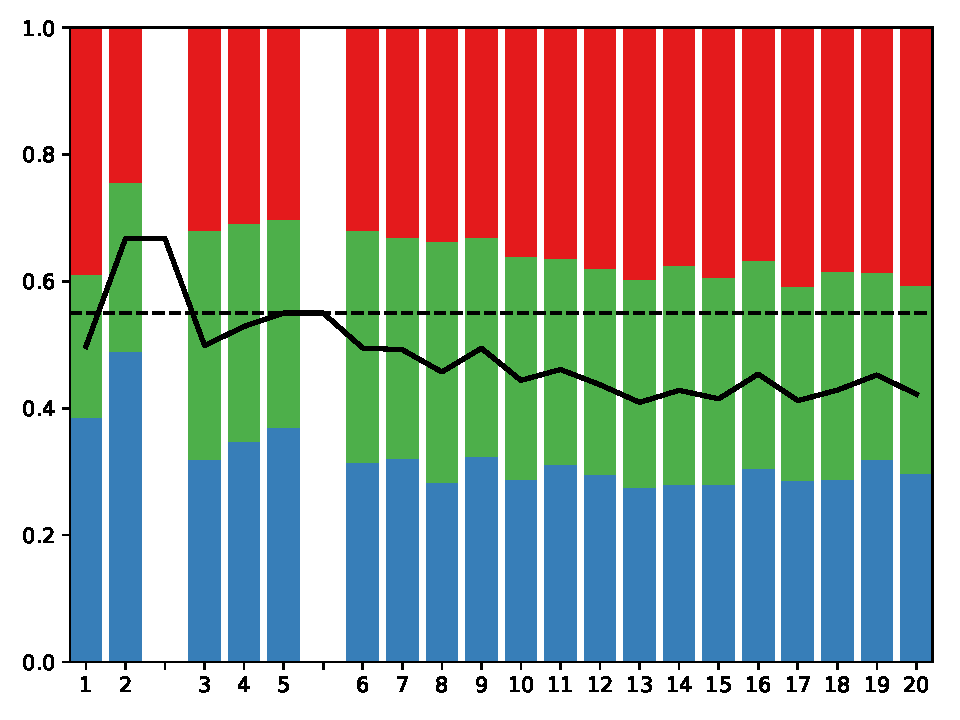
\includegraphics[width=.5\textwidth]{plots/4.pdf}
    \caption{2000 episodes, 100 MCTS iterations}
\end{figure}

On the other hand, with both a large dataset and a large number of MCTS
iterations, the model learns very quickly, reaching the optimal policy after
only training 5 times, in our example.

\begin{figure}[h!]
    \centering
    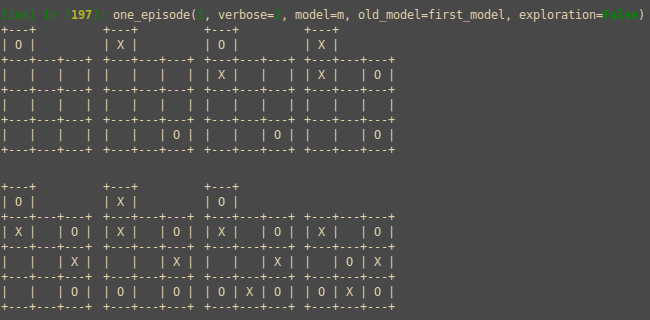
\includegraphics[width=.8\textwidth]{plots/tictactoe.png}
    \caption{Simulated game between the trained model and the initial model.
        Regardless of the simple nature of the game, the used strategy displays
        a clear improvement in predictive power, and an abilitiy to think multiple
    steps into the future.}
\end{figure}

\end{document}
